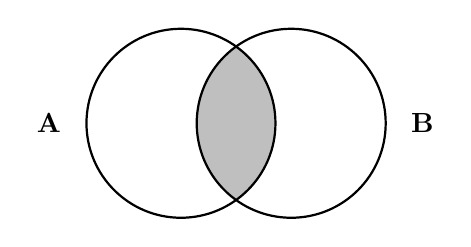
\begin{tikzpicture}[scale=1]

    % Use a scope to restrict the fill to the intersection of the two circles
    \begin{scope}
        % Clip the drawing area to the left circle
        \clip (0,0) circle (1.2);
        
        % Web renderers often fail with 'patterns'. 
        % Using a solid fill like gray!50 is web-safe and renders correctly everywhere.
        \fill[gray!50] (1.4,0) circle (1.2);
    \end{scope}

    % Draw the outline of the left circle
    \draw[thick] (0,0) circle (1.2);

    % Draw the outline of the right circle
    \draw[thick] (1.4,0) circle (1.2);

    % Place label A to the left of the left circle
    \node[left] at (-1.4, 0) {\textbf{A}};

    % Place label B to the right of the right circle
    \node[right] at (2.8, 0) {\textbf{B}};

\end{tikzpicture}